% 대한산업공학회 제출용 한글 원고 (XeLaTeX + kotex로 컴파일)
%   xelatex apiems2026_korean.tex  (2회)
% 기술 용어는 자연스러움을 위해 영어를 그대로 사용한다.
\documentclass[11pt,a4paper]{article}
\usepackage[margin=25mm]{geometry}
\usepackage{kotex}
\usepackage{amsmath,amssymb}
\usepackage{graphicx}
\graphicspath{{figures/}}
\usepackage{float}
\usepackage{booktabs,tabularx}
\usepackage[font=small,labelfont=bf]{caption}
\usepackage{setspace}
\setstretch{1.25}
\usepackage[hidelinks]{hyperref}
\setlength{\parindent}{1em}

\title{\vspace{-8mm}\textbf{도착 시각(release time)과 soft due date를 갖는\\
컴파운드 트럭 크로스도킹 스케줄링:\\
병목 유도(bottleneck-guided) Iterated Local Search}}
\author{김영수\thanks{제1저자.} \quad 권상진\thanks{교신저자. Email: [지도교수 이메일 기입].}\\
\small 연세대학교 인공지능학과, 서울}
\date{}

\begin{document}
\maketitle
\vspace{-4mm}

\begin{abstract}
\noindent
컴파운드 트럭(compound truck)이 부분 하역된 뒤 특정 목적지의
출고 운송 트럭으로 전환되는 다중 도어 크로스도킹 스케줄링 문제를 다룬다.
기존 컴파운드 트럭 모델은 모든 트럭이 시각 0에 도착한다고 가정하고 총 작업완료시간
(makespan)만 최소화한다. 본 연구는 트럭별 도착 시각(release time)과, 위반을 허용하되
지연 비용을 부과하는 soft due date를 도입하고, makespan과 총 납기지연(tardiness)의
합을 최소화하는 문제로 확장한다. 문제를 mixed-integer
program과 CP-SAT 모형으로 정식화하고, 서로 겹치지 않는 train, tuning, test seed 집합을 사용한 재현 가능한
실험 프로토콜을 제시한다. 제안 방법 VAA-GILS는 Vogel식 구성(construction),
best-improvement descent, 병목(bottleneck) 유도 연산자, simulated annealing
acceptance, kick restart를 결합한 iterated local search이다. CP-SAT 기준해가
존재하는 실험 조건에서 VAA-GILS는 해당 CP-SAT incumbent 대비 0.1--0.6\% 이내의 목적값을 1초
미만에 얻었고(CP-SAT는 76--376초), 소형 무(無)시간창 인스턴스에서는 증명된
최적해와 일치하였다. CP-SAT가 600초 내 실행 가능해를 찾지 못한 대형 시간창
조건에서는 비교 방법 가운데 가장 좋은 해를 제공하였다. Ablation 결과, 성능 향상은
descent, 병목 유도 연산자, restart라는 결정론적 구조에서 비롯되며, learned
operator selection(tabular Q-learning, transfer DQN)은 동일 예산에서 uniform
sampling을 능가하지 못하였다.

\smallskip
\noindent\textbf{주제어:} cross-docking; compound truck; release time; soft due date;
iterated local search; constraint programming
\end{abstract}

\section{서론}

크로스도킹은 입고 화물을 창고에 보관하지 않고 곧바로 출고 트럭으로 환적하여
재고와 리드타임을 줄이는 물류 방식이다~\cite{boysen2010,vanbelle2012}. 컴파운드
트럭 변형에서는 한 대의 트럭이 두 역할을 겸한다. 다른 목적지의 화물을 하역하되
한 목적지의 화물은 유지하고, 이후 해당 목적지의 화물을 다른 컴파운드 트럭들로부터 받아
출고 운송 트럭으로 출발한다~\cite{joo2013,shahmardan2020}. 부분 하역은 makespan을 크게
줄일 수 있으나, 기존 모델은 모든 트럭이 시각 0에 가용하다고 가정하며 due date
성능 지표가 없다.

도착 시각(release time), 시간창(time window), 납기지연(tardiness)은 일반 크로스도킹 스케줄링에서 이미
연구되어
왔다~\cite{vanbelle2013,assadi2016,bodnar2017,molavi2018,rijal2019,li2026};
불확실하거나 불완전한 도착 정보는~\cite{larbi2011,konur2013,konurcost2013,ladier2016,xi2020}에서
다룬다. 그러나 이들은 트럭을 순수 입고 또는 출고 트럭으로 고정한다. 컴파운드
트럭 설정은 다르다. 트럭은 부분 하역 후 한 목적지의 화물을 유지하고, 해당 목적지로
들어오는 이송 화물을 기다린 뒤 비로소 출고 운송 트럭으로 출발한다. 이 부분 하역 변환은
하나의 precedence chain(도착 $\to$ 부분 하역 $\to$ 유지 화물 $\to$
이송 대기 $\to$ 출고)을 만든다. 따라서 한 트럭의 늦은 도착은
해당 트럭의 이송 화물에 의존하는 모든 출고 운송 트럭으로 전파되고, soft due date는 이 연쇄
지연을 tardiness 비용으로 바꾼다. 본 연구의 기여는 이 상호작용 --- 알려진
release time과 soft due date가 부분 하역 후 출고 운송 트럭으로 전환되는 과정과 결합되는 방식 --- 을
정식화하고 분석하는 것이다.

본 연구의 기여는 세 가지다. 첫째, 독립적인 스케줄 평가기와 일치하는 MILP 및
CP-SAT 정식화를 제공한다. 둘째, 기존 VAA construction과 generic neighborhood에
full best-improvement descent, makespan-critical 및 tardiness-critical 연산자,
restart를 더한 VAA-GILS를 제안한다~\cite{shahmardan2020}. 셋째, 통제된
ablation으로 성능 향상이 탐색 엔진에서 비롯되는지 학습 기반 연산자 선택에서
비롯되는지를 구분한다. 후자는 동일 예산의 균등 선택 방식을 능가하지 못하였다.

\section{문제 정의}

$I$, $F$, $D$, $K$, $M$을 각각 컴파운드 트럭, 출고 트럭, 목적지, 상품 종류,
도어의 집합이라 하고 $|I|+|F|=|D|$, $|I|\le|M|$이라 하자. 컴파운드 트럭 $i$는
목적지 $d$행 상품 $k$를 $f_{idk}$ 단위 싣는다. 단위 처리시간 $t_k$에 대해
$h_{id}=\sum_k f_{idk}t_k$, $H_i=\sum_d h_{id}$로 둔다. 각 컴파운드 트럭은 유지할
목적지 하나와 도어 하나를 고르며 도어당 컴파운드 최대 1대이다. 각 출고 트럭은
남은 목적지 하나와 도어를 고르고, 같은 도어의 출고 트럭은 작업 순서를 정한다. 따라서
각 목적지에는 정확히 하나의 운송 트럭이 배정된다. 트럭 $q\in I\cup F$의 release
time을 $r_q$로 나타낸다. 따라서 $r_i$는 컴파운드 트럭 $i\in I$가 도어 작업을
시작할 수 있는 가장 이른 시각이고, $r_f$는 출고 트럭 $f\in F$가 도어 작업을
시작할 수 있는 가장 이른 시각이다. 트럭 $q$는 $r_q$ 이전에 시작할 수 없고 soft
due date $\bar d_q$를 갖는다. 완료 시각을 $C_q$,
makespan을 $C_{\max}=\max_q C_q$, tardiness를 $T_q=\max\{0,C_q-\bar d_q\}$라 할
때 목적함수는
\begin{equation}
\min\ J=C_{\max}+\lambda\sum_{q\in I\cup F}T_q,\qquad \lambda=1.
\label{eq:obj}
\end{equation}

시간 계산은 물리적 작업 순서를 따른다. 컴파운드 트럭 $i$가 목적지 $d$의 화물을 유지하면 하역은
$U_i=r_i+DE_i+H_i-h_{id}$에 끝난다. 운송 트럭은 화물을 보내는 모든 트럭이 하역을
마치고 해당 화물의 도어 간 이송이 끝난 뒤에야 적재할 수 있다. 출고 운송 트럭은
추가로 자신의 release와 도어의 선행 점유가 끝나기를 기다린다. 그 시점에 도어 작업을
시작하여 진입($DE_f$), 적재, 출차($DL_f$)를 차례로 수행한다. 목적지 $d$의 적재시간은
$L_d=\sum_i h_{id}$이며 진입·출차 시간은 별도로 더한다.

\paragraph{MILP 요약.} 이진 변수 $x_{idm}$은 컴파운드 트럭 $i$를 유지 목적지
$d$·도어 $m$에, $z_{fdm}$은 출고 트럭 $f$를 배정한다. 운송 트럭 및 컴파운드 트럭의
도어 배정은 $\sum_{d,m}x_{idm}=1$, $\sum_{d,m}z_{fdm}=1$,
$\sum_{i,m}x_{idm}+\sum_{f,m}z_{fdm}=1$($\forall d$), $\sum_{i,d}x_{idm}\le1$을
만족한다. 모든 입고 이송의 선후관계는 big-$M$ implication으로 부과한다
(예: $C_i\ge U_j+t_{nm}+L_d+DL_i-B(2-x_{idm}-X_{jn})$). CP-SAT 모형은 big-$M$
disjunction을 enforcement literal로 대체하고 시간을 0.01 단위로 정수화한다.
모든 배정을 고정하면 독립 evaluator의 완료 시각이 재현되어 model fidelity가
확인된다.

\section{VAA-GILS}

\textbf{초기해 구성.} VAA는 Vogel식 regret으로 유지 목적지를 정하고, 완료 시각
우선순위에 따라 출고 목적지를 배정한 뒤 완료 예정 시각이 가장 이른 도어에 삽입한다.
모든 완료 예정 시각 계산에는 release time을 반영한다.

\textbf{Descent.} 세 무브군(출고 트럭 재배치, 컴파운드 트럭의 도어 교환/빈 도어 이동, 두
트럭 목적지 스왑)에 대한 best-improvement 지역탐색으로, local optimum에서
종료한다. 초기해·모든 신규 incumbent·최종해에 적용한다.

\textbf{반복 탐색.} 1{,}000회 반복한다. 선택 정책이 연산자 하나를
뽑아 현재 해에서 후보를 생성하고, 후보가 전역 best를 개선하면 descent를 적용해
incumbent를 갱신한다. acceptance는 초기 온도 $T_0=\max\{1,\,0.05\,J(s_0)\}$,
기하 냉각 $T\leftarrow0.995\,T$의 simulated annealing이다. 30회 연속 개선이 없으면 현재 최선해에서
random kick 3회로 재시작하고 $T\leftarrow\max\{T,\,0.02\,J(s^*)\}$로 reheat한다.

\textbf{Operator pool.} 기존 generic neighborhood 7종에, 현재 병목을 먼저 식별한
뒤 그 주변을 best-of로 탐색하는 guided 연산자 4종(critical door/truck 및 most
tardy truck 기준)을 더한다. selection policy는 plug-in이며 기본값은 uniform
random이다. learned policy(tabular Q-learning, transfer DQN)는 ablation
목적으로만 평가하며 제안 방법의 일부가 아니다.

\section{실험 설계}

세 규모 $(|I|,|D|,|M|)$: S $(6,9,6)$, M $(12,18,12)$, L $(20,30,20)$을 사용한다.
flow는 상품 3종에 대해 $[0,20]$의 균등 정수, $t_k\sim U[1,5]$, 도어는
$100\times100$ 랜덤 배치이다. 시간창 수준은 none/medium/tight이며, medium과
tight에서 $r\sim U[0,\rho H]$, $\bar d=r+\delta H$, $(\rho,\delta)=(0.25,0.60)$,
$(0.50,0.35)$이다.

seed는 서로소인 train/tuning/test 풀로 분리한다. 주 분석은 셀당 독립 생성한
test 인스턴스 20개와 stochastic replication 5회를 사용한다. 먼저 인스턴스별로
replication을 평균한 뒤, 짝지은 인스턴스 평균에 양측 Wilcoxon signed-rank test를
적용한다(replication은 독립 관측으로 취급하지 않는다). GILS는 1{,}000회
반복한다. CP-SAT는 인스턴스당 1회, 8 thread로 S 300초, M/L 600초 실행한다.
S-none 5개만 최적이 증명되며, 나머지 exact 비교는 CP-SAT incumbent를 기준으로
한다. baseline은 VAA, SA-RL5 재구현~\cite{shahmardan2020}, 그리고 uniform/
tabular-Q/transfer-DQN selection의 GILS이다. 주 지표는 모든 방법과 예산 및 CP-SAT를
포함하여 관측된 최선해에 대한 인스턴스별 gap $\Delta_{bo}$이다.

\section{실험 결과}

표~\ref{tab:quality}가 test 결과를 요약한다. GILS는 모든 실험 조건에서 평균 gap이
0.3\% 미만이고, 기준해가 있는 조건에서 CP-SAT incumbent 대비 0.1--0.6\% 이내이다.
S-none 5개는 최적이 증명되었다. 대형 시간창 조건에서 CP-SAT는 600초 내 실행 가능해를
찾지 못하므로, 해당 조건에서는 CP-SAT 기준이 아니라 비교 방법에 대한 우세를
주장한다.

\begin{table}[t]
\centering
\caption{평균 test 목적값과 관측된 최선해 대비 gap. S-none만 최적 증명.}
\label{tab:quality}
\small
\begin{tabular}{@{}lrrrrrrrrr@{}}
\toprule
& \multicolumn{3}{c}{No windows} & \multicolumn{3}{c}{Medium} & \multicolumn{3}{c}{Tight}\\
\cmidrule(lr){2-4}\cmidrule(lr){5-7}\cmidrule(lr){8-10}
규모 & VAA & GILS & $\Delta_{bo}$ & VAA & GILS & $\Delta_{bo}$ & VAA & GILS & $\Delta_{bo}$\\
\midrule
S & 1497.5 & 1411.8 & 0.16\% & 5447.5 & 5255.7 & 0.08\% & 9276.8 & 9010.8 & 0.09\%\\
M & 3030.9 & 2928.9 & 0.29\% & 23025.5 & 22526.4 & 0.29\% & 38903.7 & 38528.0 & 0.19\%\\
L & 5492.3 & 5388.4 & 0.27\% & 55611.1 & 54846.4 & 0.10\% & 119671.9 & 118901.4 & 0.08\%\\
\bottomrule
\end{tabular}
\end{table}

SA-RL5가 정의된 셀에서 GILS $<$ SA-RL5 $<$ VAA 순서가 성립한다. 제안 방법의
default selector인 uniform 기준으로, 짝지은 검정에서 GILS(uniform)는 VAA를 평균
2.65\%($n=180$, $p<10^{-4}$), SA-RL5를 1.38\%($n=60$, $p<10^{-4}$) 능가한다.
tabular Q-learning과 transfer DQN의 selector 비교는 5.1절에서 다룬다. GILS의 평균 실행 시간은 S/M/L에서 0.11, 0.52, 2.3초이고,
CP-SAT는 각각 76, 237, 376초이다.

\subsection{Ablation 및 operator selection}

generic pool에 makespan-critical 연산자를, 이어서 tardiness-critical 연산자를
더하면 모든 실험 조건에서 gap이 낮아진다. generic→critical 개선은 0.114\%p($p<10^{-4}$),
critical→full은 0.047\%p($p=0.0001$)이다(그림~\ref{fig:operators}).

\begin{figure}[H]
\centering
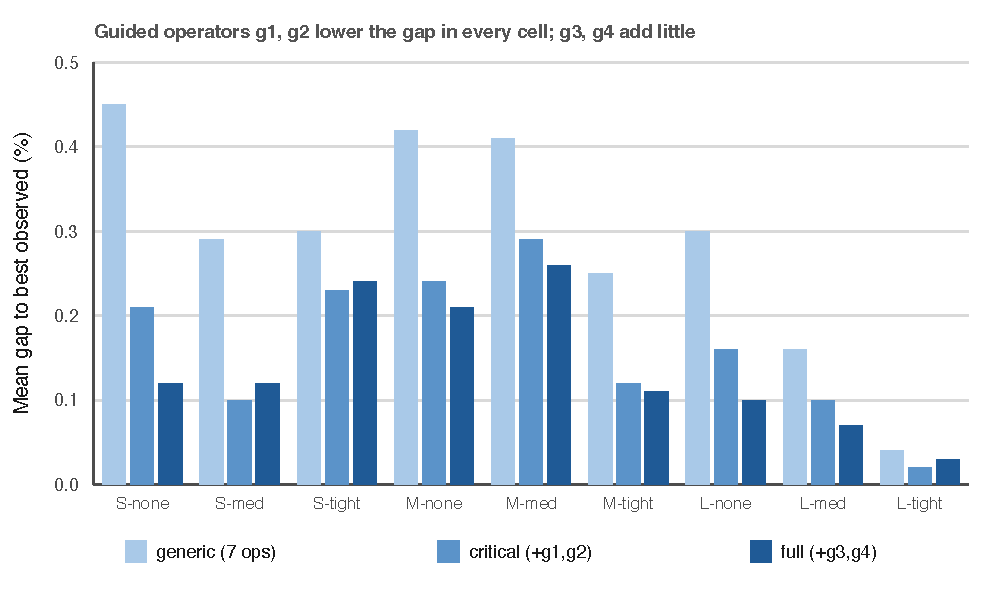
\includegraphics[width=0.8\columnwidth]{fig2_operator_pool.pdf}
\caption{operator pool별 관측된 최선해 대비 gap.}
\label{fig:operators}
\end{figure}

Leave-one-out 결과, descent의 기여가 가장 크다(제거 시 0.156\%p 악화,
$p<10^{-4}$). restart 제거는 0.069\%p($p<10^{-4}$)이다. VAA initialization은
통계적으로 유의한 pooled 효과가 없고(0.022, $p=0.114$), greedy acceptance가 이
엔진에서 SA보다 근소하게 낫다. 즉 construction과 확률적 acceptance는 성능의
원천이 아니다(그림~\ref{fig:components}).

\begin{figure}[H]
\centering
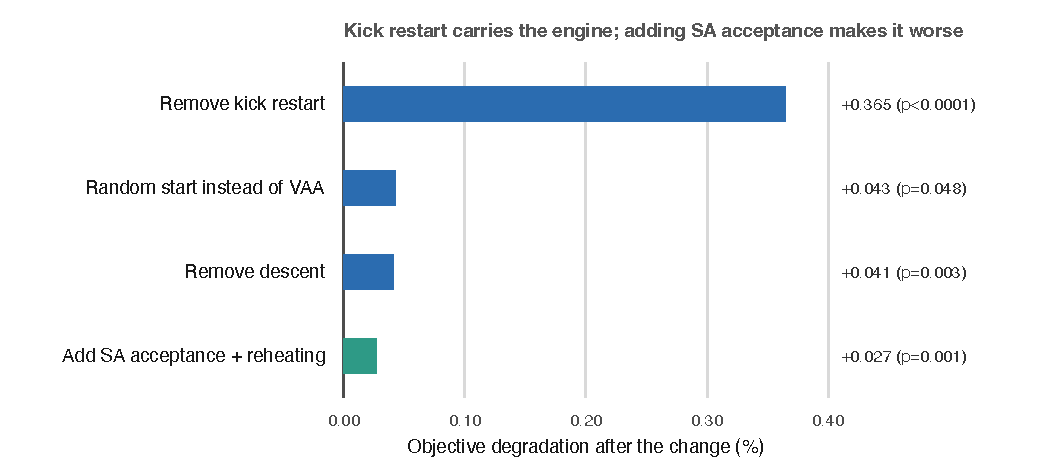
\includegraphics[width=0.8\columnwidth]{fig3_component_ablation.pdf}
\caption{컴포넌트 제거 시 목적값 악화율.}
\label{fig:components}
\end{figure}

학습 기반 연산자 선택의 추가 효과도 작다. 1{,}000회에서 tabular Q-learning은
uniform과 $-0.01$\%p 차이($p=0.150$), DQN은 uniform보다 0.11\%p
열세이다($p<10^{-4}$)~\cite{watkins1992,mnih2015}. 50--3{,}000회 예산에서 어떤
어떤 학습 기반 선택기도 일관되게 앞서지 못하며, 이러한 부정적 결과는 무시간창 셀에서도
성립하므로 시간창 확장 때문에 나타난 결과가 아니다(그림~\ref{fig:selector}).

\begin{figure}[H]
\centering
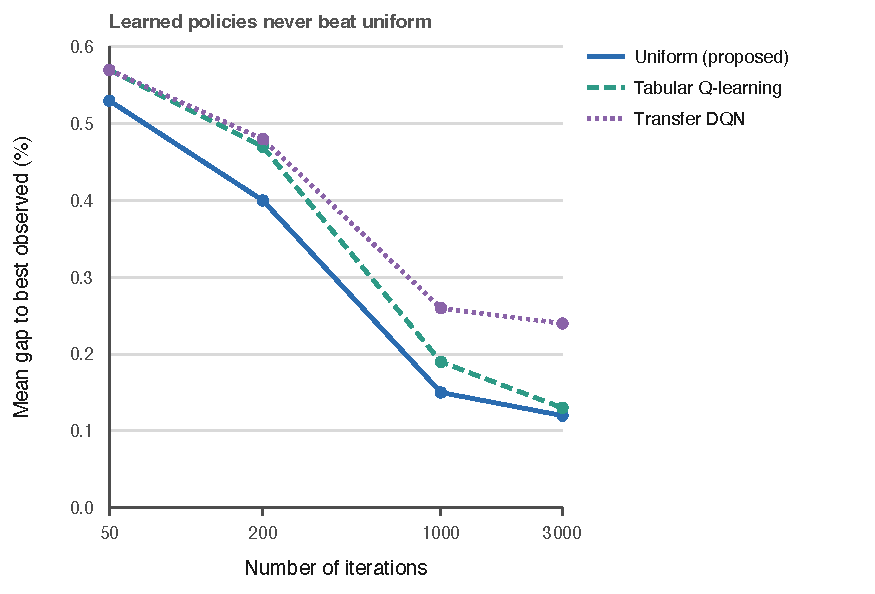
\includegraphics[width=0.72\textwidth]{fig1_selector_budget.pdf}
\caption{iteration budget에 따른 관측된 최선해 대비 gap. tabular는 최대
예산에서만 uniform보다 근소하게 앞서고, transfer DQN은 이기지 못한다.}
\label{fig:selector}
\end{figure}

\subsection{Tardiness-weight 민감도}

식~\eqref{eq:obj}이 시간 단위 성분 둘을 합치므로, tuning 풀에서
$\lambda\in\{0,0.25,0.5,1,2,4,8\}$을 스윕한다. 물리적 makespan과 총 tardiness를
기록하고 인스턴스별로 두 지표를 min--max 정규화한 뒤 평균한다
(그림~\ref{fig:lambda}). tardiness 감소의 대부분은 $\lambda=0$에서 $1$ 사이에서
일어나고 이후에는 증가 폭이 둔화된다. 전체 스윕 구간에서 평균 makespan은 약 1\% 상승, 평균
tardiness는 2--3\% 하락한다. $\lambda=1$을 채택한다: 완만한 makespan 비용으로
tardiness가 거의 최소에 이르고, 두 시간 성분에 동일 가중을 준다는 해석이
자연스럽다. 이 스윕은 test가 아닌 tuning 인스턴스를 사용한 설계 정당화이며 post-hoc
parameter 선택이 아니다.

\begin{figure}[H]
\centering
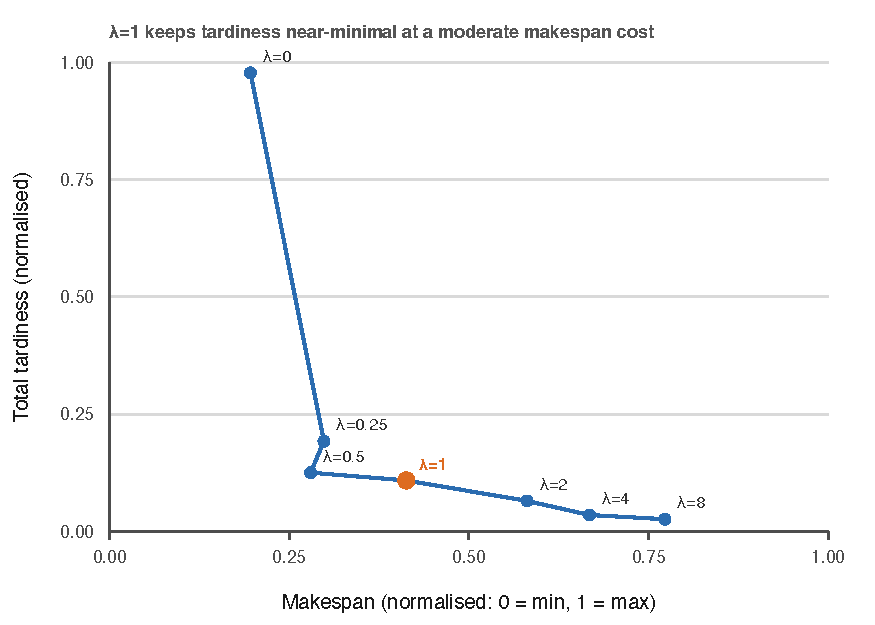
\includegraphics[width=0.72\textwidth]{fig4_lambda_tradeoff.pdf}
\caption{tuning 인스턴스에서의 정규화된 makespan--tardiness trade-off.}
\label{fig:lambda}
\end{figure}

\section{논의 및 결론}

알려진 release time과 soft due date는 컴파운드 트럭 스케줄을 실질적으로 바꾼다.
출고 운송 트럭은 화물을 보내는 트럭의 이송 완료와 자신의 가용 시각을 함께 기다려야 하고, 도어 배정은
makespan과 tardiness를 결합한다. VAA-GILS는 이 확장을 빠르게 처리하고 가용한
CP-SAT 기준해에 근접한다. 결과의 해석 범위는 다음과 같이 제한한다. S-none만 최적이 증명되고,
대형 시간창 조건에서는 최적성이 아니라 비교 방법에 대한 우세만을 주장한다.

Ablation은 성능의 해석을 바꾼다. best-improvement descent, guided move, restart가
탐색을 이끈다. 이 구조가 갖춰지면 uniform selector가 동일 예산에서 learned
대안만큼 효과적이다. SA acceptance와 reheating은 기저 SA-RL5 framework와의
comparability를 위해 유지하였으나, ablation은 본 설정에서 이들이 해 품질에
필수적이지 않음을 보인다. 이는 학습이 일반적으로 무의미하다는 뜻이 아니다; online
arrival, 이질적 인스턴스, 더 큰 operator pool은 adaptation의 역할을 키울 수 있다.
향후에는 도착 정보가 실시간으로 공개되는 문제, robust schedule, 더 강한 lower bound,
산업 데이터를 활용한 사례 연구가 필요하다.

\section*{생성형 AI 사용 명시}
원고 준비 과정에서 저자들은 언어 교정, 원고 구성, 참고문헌 확인, 그리고 계산
코드 개발·검토 보조를 위해 OpenAI Codex(GPT-5)와 Claude Code(Anthropic)를
사용하였다. 저자들은 모든 참고문헌·정식화·코드·결과·해석을 검토·검증하였으며
내용에 대한 전적인 책임을 진다.

\begin{thebibliography}{99}\small
\bibitem{assadi2016} M. T. Assadi and M. Bagheri, ``Differential evolution and population-based simulated annealing for truck scheduling,'' \emph{Computers \& Industrial Engineering}, vol. 96, pp. 149--161, 2016.
\bibitem{bodnar2017} P. Bodnar, R. de Koster, and K. Azadeh, ``Scheduling trucks in a cross-dock with mixed service mode dock doors,'' \emph{Transportation Science}, vol. 51, no. 1, pp. 112--131, 2017.
\bibitem{boysen2010} N. Boysen and M. Fliedner, ``Cross dock scheduling: Classification, literature review and research agenda,'' \emph{Omega}, vol. 38, pp. 413--422, 2010.
\bibitem{joo2013} C. M. Joo and B. S. Kim, ``Scheduling compound trucks in multi-door cross-docking terminals,'' \emph{International Journal of Advanced Manufacturing Technology}, vol. 64, pp. 977--988, 2013.
\bibitem{konur2013} D. Konur and M. M. Golias, ``Analysis of different approaches to cross-dock truck scheduling with truck arrival time uncertainty,'' \emph{Computers \& Industrial Engineering}, vol. 65, no. 4, pp. 663--672, 2013.
\bibitem{konurcost2013} D. Konur and M. M. Golias, ``Cost-stable truck scheduling at a cross-dock facility with unknown truck arrivals,'' \emph{Transportation Research Part E}, vol. 49, no. 1, pp. 71--91, 2013.
\bibitem{ladier2016} A.-L. Ladier and G. Alpan, ``Robust cross-dock scheduling with time windows,'' \emph{Computers \& Industrial Engineering}, vol. 99, pp. 16--28, 2016.
\bibitem{larbi2011} R. Larbi, G. Alpan, P. Baptiste, and B. Penz, ``Scheduling cross docking operations under full, partial and no information on inbound arrivals,'' \emph{Computers \& Operations Research}, vol. 38, no. 6, pp. 889--900, 2011.
\bibitem{li2026} Y. Li, M. Mohammadi, X. Zhang, Y. Lan, and W. van Jaarsveld, ``Integrated trucks assignment and scheduling with mixed service mode docks,'' \emph{European Journal of Operational Research}, vol. 333, no. 1, pp. 117--137, 2026.
\bibitem{molavi2018} D. Molavi, A. Shahmardan, and M. S. Sajadieh, ``Truck scheduling in a cross docking systems with fixed due dates and shipment sorting,'' \emph{Computers \& Industrial Engineering}, vol. 117, pp. 29--40, 2018.
\bibitem{rijal2019} A. Rijal, M. Bijvank, and R. de Koster, ``Integrated scheduling and assignment of trucks at unit-load cross-dock terminals,'' \emph{European Journal of Operational Research}, vol. 278, no. 3, pp. 752--771, 2019.
\bibitem{shahmardan2020} A. Shahmardan and M. S. Sajadieh, ``Truck scheduling in a multi-door cross-docking center with partial unloading,'' \emph{Computers \& Industrial Engineering}, vol. 139, Art. 106134, 2020.
\bibitem{mnih2015} V. Mnih et al., ``Human-level control through deep reinforcement learning,'' \emph{Nature}, vol. 518, pp. 529--533, 2015.
\bibitem{vanbelle2012} J. Van Belle, P. Valckenaers, and D. Cattrysse, ``Cross-docking: State of the art,'' \emph{Omega}, vol. 40, no. 6, pp. 827--846, 2012.
\bibitem{vanbelle2013} J. Van Belle, P. Valckenaers, G. Vanden Berghe, and D. Cattrysse, ``A tabu search approach to the truck scheduling problem with multiple docks and time windows,'' \emph{Computers \& Industrial Engineering}, vol. 66, no. 4, pp. 818--826, 2013.
\bibitem{watkins1992} C. J. C. H. Watkins and P. Dayan, ``Q-learning,'' \emph{Machine Learning}, vol. 8, pp. 279--292, 1992.
\bibitem{xi2020} X. Xi, C. Liu, Y. Wang, and L. H. Lee, ``Two-stage conflict robust optimization models for cross-dock truck scheduling under uncertainty,'' \emph{Transportation Research Part E}, vol. 144, Art. 102123, 2020.
\end{thebibliography}

\end{document}
